% Fichier généré automatiquement par tools/generate_corrections.py.
% Source : STAT/STAT-03-Demarche/06_TR/06_TR.tex
% Statut : partiel (1/4 question(s) renseignée(s), 1 reprise(s)).
\begin{corrigebox}[Corrigé partiel extrait de la banque]
\CorrigeQuestion{1}
\CorrigeSource{Réponse reprise d'un exercice homonyme de la banque ; la provenance exacte est indiquée dans le commentaire du fichier.}
% Réponse reprise de : DYN/DYN-05-Methode/06_TR/06_TR.tex
\par\medskip\begin{center}\captionsetup{type=figure}
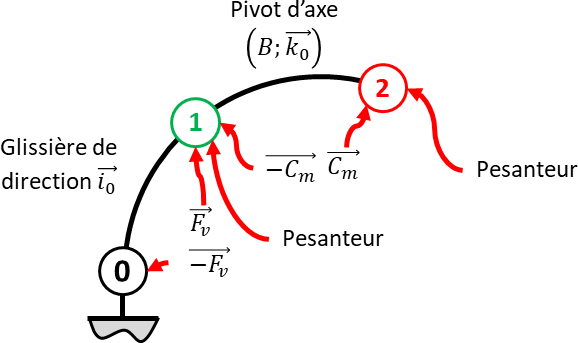
\includegraphics[width=.7\linewidth]{../../../DYN/DYN-05-Methode/06_TR/images/06_TR_02_Cor}
\end{center}\par\medskip
\CorrigeQuestion{2}
\CorrigeACompleter{Aucun élément de réponse n'est présent dans la source d'origine pour cette question.}
\CorrigeQuestion{3}
\CorrigeACompleter{Aucun élément de réponse n'est présent dans la source d'origine pour cette question.}
\CorrigeQuestion{4}
\CorrigeACompleter{Aucun élément de réponse n'est présent dans la source d'origine pour cette question.}
\end{corrigebox}
